\section{ACTVIVIDAD 01: Importación de Datos usando el Wizard - SQL MANAGMENT} 

1. Primeramente crearemos una base de datos llamada BDTEST.
	\begin{center}
	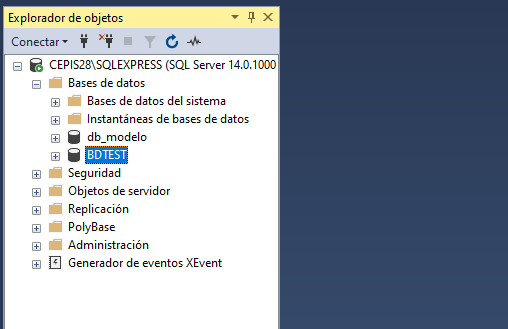
\includegraphics[width=\columnwidth]{images/task1/img1}
	\end{center}	


2. Ahora importaremos nuestra base de datos desde AdventureWorks.
	\begin{center}
	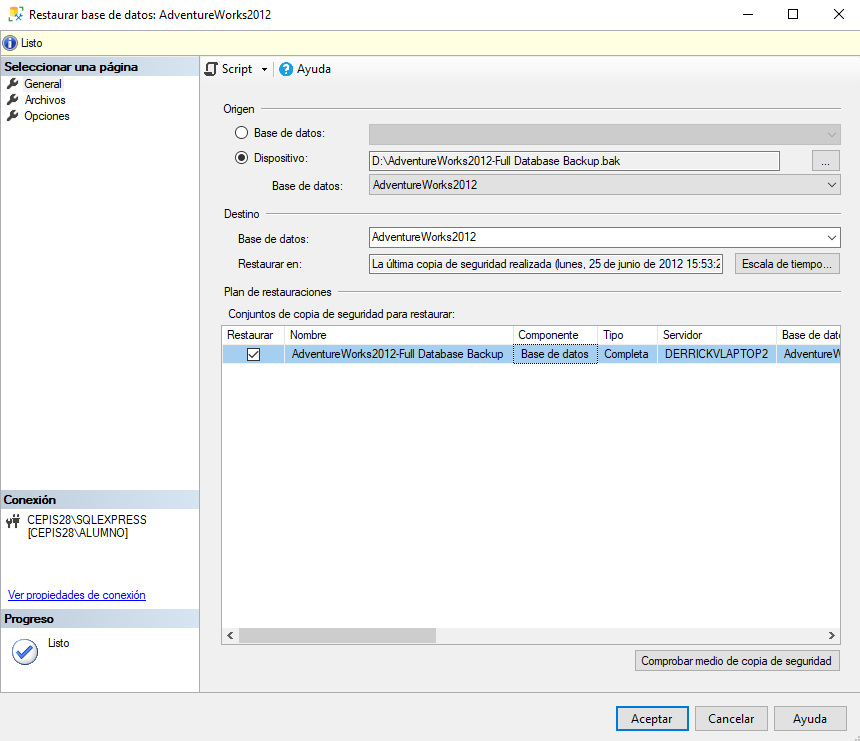
\includegraphics[width=\columnwidth]{images/task1/img2}
	\end{center}	

3. Next y escribir el Servidor y seleccionar la base de datosg.
	\begin{center}
	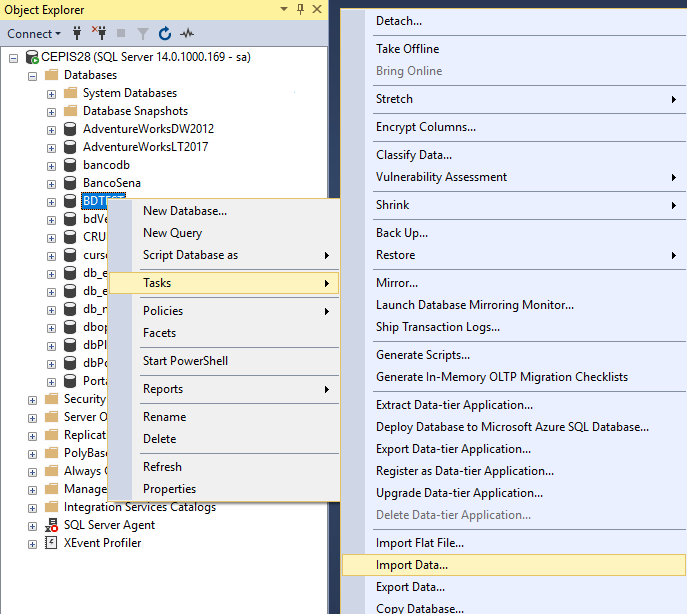
\includegraphics[width=\columnwidth]{images/task1/img3}
	\end{center}	

4. Data Source: La base de donde vamos a importar - Destination: La Base donde vamos a cargar la datas.
	\begin{center}
	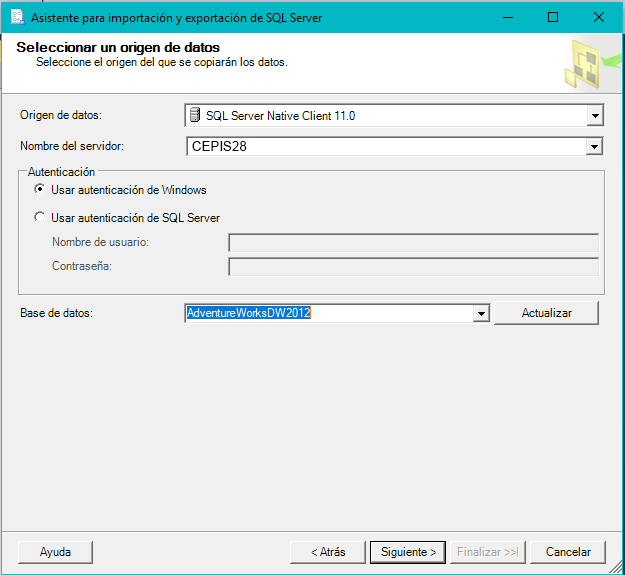
\includegraphics[width=\columnwidth]{images/task1/img4}
    \end{center}	
    
	\begin{center}
	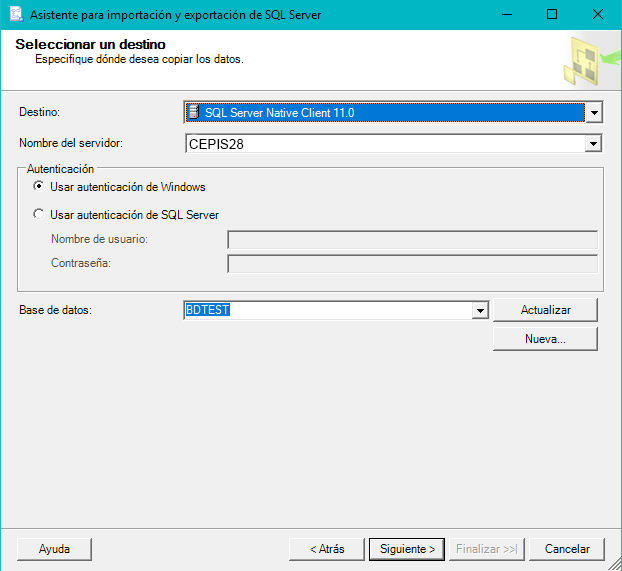
\includegraphics[width=\columnwidth]{images/task1/img5}
    \end{center}	
    
	\begin{center}
	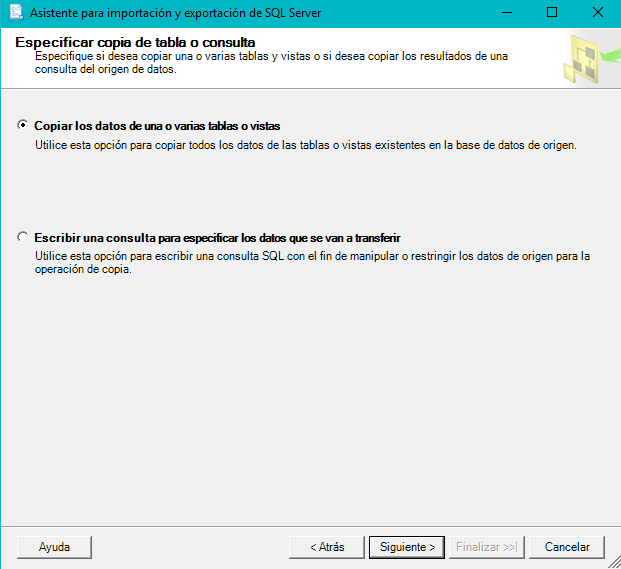
\includegraphics[width=\columnwidth]{images/task1/img6}
    \end{center}	
    
	\begin{center}
	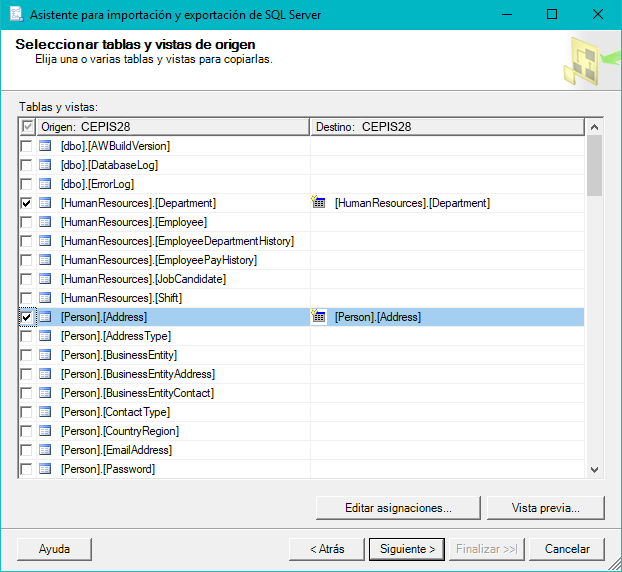
\includegraphics[width=\columnwidth]{images/task1/img7}
    \end{center}	
    
	\begin{center}
	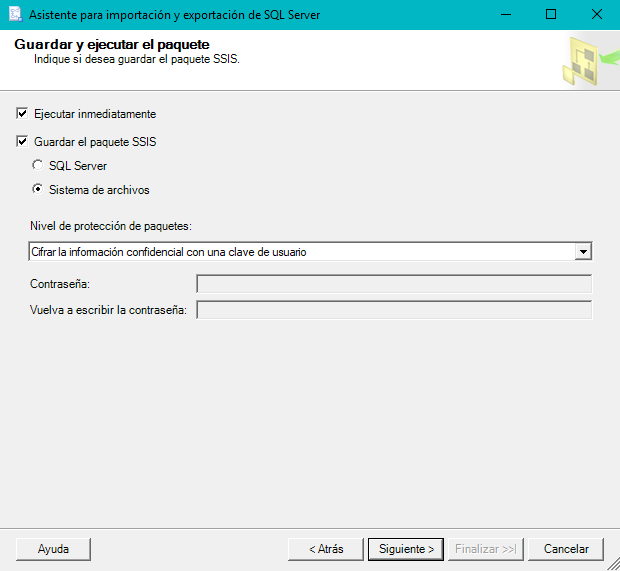
\includegraphics[width=\columnwidth]{images/task1/img8}
    \end{center}	
    
	\begin{center}
	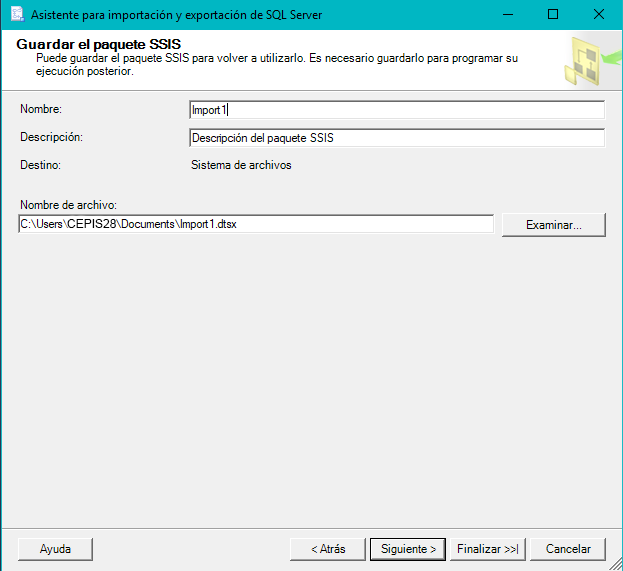
\includegraphics[width=\columnwidth]{images/task1/img9}
    \end{center}	
    
	\begin{center}
	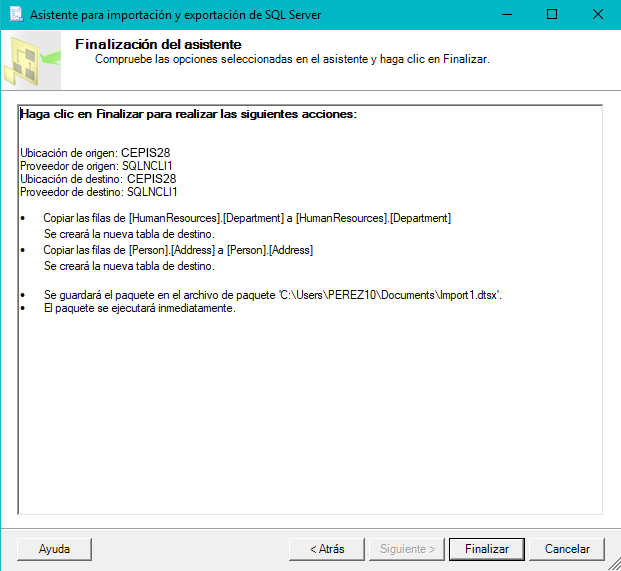
\includegraphics[width=\columnwidth]{images/task1/img10}
    \end{center}	
    
	\begin{center}
	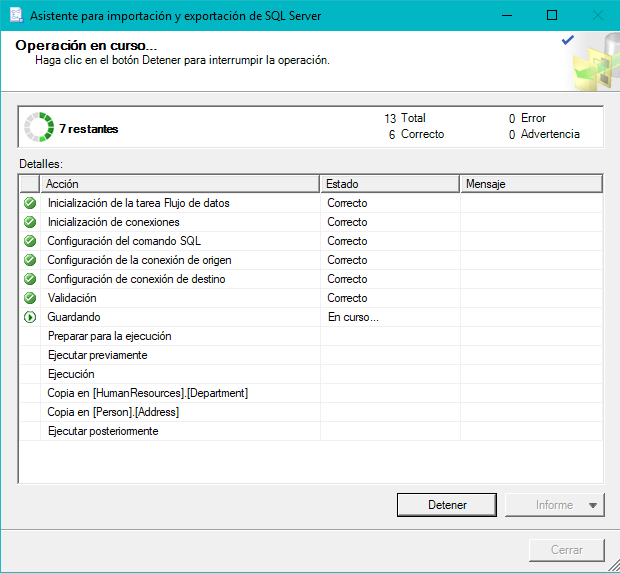
\includegraphics[width=\columnwidth]{images/task1/img11}
    \end{center}	
    
5. Al final veremos un resumen de la ejecución.
	\begin{center}
	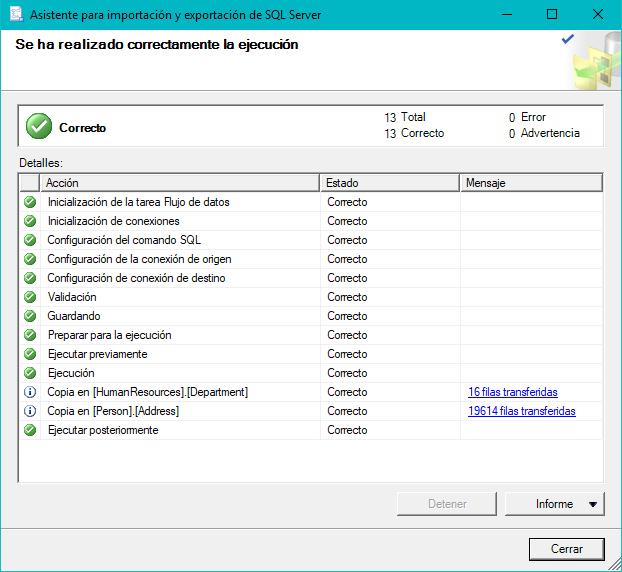
\includegraphics[width=\columnwidth]{images/task1/img12}
	\end{center}	